\documentclass[11pt,a4paper]{article}
\usepackage[utf8]{inputenc}
\usepackage[T1]{fontenc}
\usepackage[margin=2.2cm]{geometry}
\usepackage{lmodern}
\usepackage{microtype}
\usepackage{amsmath,amssymb}
\usepackage[table]{xcolor}
\usepackage{booktabs}
\usepackage{tabularx}
\usepackage{float}
\usepackage{enumitem}
\usepackage[most]{tcolorbox}
\usepackage{fancyhdr}
\usepackage{needspace}
\usepackage{titlesec}
\usepackage{tikz}
\usetikzlibrary{arrows.meta,positioning,calc,shapes.geometric,fit}
\usepackage[colorlinks=true,linkcolor=blue!60!black,urlcolor=blue!60!black]{hyperref}

\setlist[itemize]{nosep,leftmargin=*,topsep=2pt,partopsep=0pt}
\setlist[enumerate]{nosep,leftmargin=*,topsep=2pt,partopsep=0pt}
\widowpenalty=10000
\clubpenalty=10000
\setlength{\parskip}{0.55em}
\setlength{\parindent}{0pt}

\definecolor{cblue}{HTML}{2B6CB0}
\definecolor{cgreen}{HTML}{2F855A}
\definecolor{cred}{HTML}{C53030}
\definecolor{corange}{HTML}{DD6B20}
\definecolor{cgray}{HTML}{718096}
\definecolor{cpurple}{HTML}{6B46C1}

\titleformat{\section}{\Large\bfseries\color{cblue}}{\thesection}{0.6em}{}
\titleformat{\subsection}{\large\bfseries\color{cblue!80!black}}{\thesubsection}{0.6em}{}

\pagestyle{fancy}
\fancyhf{}
\lhead{\small Paper 10 explained simply}
\rhead{\small Aljalbout et al., arXiv 2510.20808}
\cfoot{\small\thepage}
\renewcommand{\headrulewidth}{0.3pt}

\newtcolorbox{idea}[1][]{colback=cblue!6,colframe=cblue!70,fonttitle=\bfseries,title={#1},boxrule=0.6pt,arc=2pt,left=6pt,right=6pt,top=4pt,bottom=4pt}
\newtcolorbox{toy}[1][]{colback=corange!7,colframe=corange!80,fonttitle=\bfseries,title={#1},boxrule=0.6pt,arc=2pt,left=6pt,right=6pt,top=4pt,bottom=4pt}
\newtcolorbox{warn}[1][]{colback=cred!6,colframe=cred!75,fonttitle=\bfseries,title={#1},boxrule=0.6pt,arc=2pt,left=6pt,right=6pt,top=4pt,bottom=4pt}
\newtcolorbox{eqbox}[1][]{colback=cgray!8,colframe=cgray!70,fonttitle=\bfseries,title={#1},boxrule=0.6pt,arc=2pt,left=6pt,right=6pt,top=4pt,bottom=4pt}
\newtcolorbox{ours}[1][]{colback=cgreen!7,colframe=cgreen!75,fonttitle=\bfseries,title={#1},boxrule=0.6pt,arc=2pt,left=6pt,right=6pt,top=4pt,bottom=4pt}

\newcommand{\Ms}{M_{\mathrm{sim}}}
\newcommand{\Mr}{M_{\mathrm{real}}}
\newcommand{\Tsim}{T_{\mathrm{sim}}}
\newcommand{\Treal}{T_{\mathrm{real}}}
\newcommand{\Osim}{O_{\mathrm{sim}}}
\newcommand{\Oreal}{O_{\mathrm{real}}}

\begin{document}
\setcounter{tocdepth}{1}

% ------------------------------------------------------------ TITLE
\begin{center}
{\LARGE\bfseries\color{cblue} Paper 10, explained from zero}\\[0.6em]
{\large \textit{The Reality Gap in Robotics: Challenges, Solutions, and Best Practices}}\\[0.5em]
Elie Aljalbout, Jiaxu Xing, Angel Romero, Iretiayo Akinola, Caelan Reed Garrett, Eric Heiden,
Abhishek Gupta, Tucker Hermans, Yashraj Narang, Dieter Fox, Davide Scaramuzza, Fabio Ramos\\
University of Zurich, NVIDIA, University of Sydney, University of Washington, University of Utah\\
arXiv 2510.20808 (23 Oct 2025), to appear in \emph{Annual Review of Control, Robotics, and
Autonomous Systems}, Vol.~9 (2026)\\[0.4em]
\textbf{Reading order \#1 of the ball-estimation chapter}
\end{center}

\begin{idea}[What this guide is]
This is a slow, step-by-step explanation of one paper, written for someone who is \emph{not}
used to academic papers, but it keeps the academic vocabulary so you can later read the
original. Every symbol is explained the first time it appears. Statements that come from the
paper are marked \textbf{(paper)}. Blue boxes are the main ideas. Orange boxes
(\textbf{Toy example}) use numbers \emph{I invented} to make an idea visible; they are
\emph{not} from the paper. Red boxes are my own critical comments, so you can tell them apart
from what the authors claim. Green boxes say what this means for \emph{our} MuJoCo ball
chapter.

I read the full text of the paper (31 pages) before writing this guide. Page and section
numbers refer to the arXiv version.
\end{idea}

\subsection*{The whole paper in six sentences}
Robots are often trained and tested inside computer simulators because simulators are cheap,
safe, fast and repeatable. But a simulator is always an \emph{approximation} of the real world,
and the difference between the two is called the \emph{reality gap}. This paper is a
\emph{survey} (a map of existing research), not a new algorithm: it splits the gap into four
families (dynamics, perception and sensing, actuation and control, system design), explains
many concrete causes inside each family, and lists a catalogue of solutions that either
\emph{reduce} the gap (make the simulator better) or \emph{overcome} it (make the robot
software tolerant to what is still wrong). It also gives formulas to \emph{measure} the gap and
the loss of performance caused by it. It contains \textbf{no new experiment and no new
numbers}; its value is vocabulary, structure and a checklist. For us it is the right first
paper, because our whole chapter is ``what happens when the perfect simulated ball state is
replaced by an imperfect simulated sensor''.

\tableofcontents
\newpage

% ============================================================ 1
\section{The story in one page}

Imagine you are teaching a robot arm to catch a rolling ball. You could do it in a real lab, but
every failed catch costs time, the ball rolls under a table, the floor is slightly different
every day, and you cannot run ten thousand attempts overnight. So you build a \emph{simulation}:
a program that computes how the ball and the arm would move according to the laws of physics,
and how a camera would see them. In the simulation you can run ten thousand attempts in an hour,
reset the ball to exactly the same starting point, and nothing breaks.

The problem is that the program is \emph{not} the world. The program says the floor friction is
$0.30$; the real floor is $0.27$ in one corner and $0.33$ in another. The program says the camera
sees the ball perfectly; the real camera sees a blurry blob, loses it when it is too close to the
wall, and delivers each image $40$ ms late. If you tune your robot until it is perfect in the
simulation, it may fail on the real floor. The distance between the two worlds is the
\textbf{reality gap}.

This paper asks four questions, and its sections answer them in order:
\begin{enumerate}
\item \textbf{What exactly is the gap, mathematically?} (Section 2 of the paper.)
\item \textbf{Where does it come from?} (Section 3.)
\item \textbf{What can we do about it?} (Section 4.)
\item \textbf{How do we measure it?} (Section 5.)
\end{enumerate}
Section 6 lists open problems.

\begin{idea}[One sentence to remember]
\emph{A simulator will never be perfect, so the goal is not to remove the gap but to know which
parts of it matter for your task, shrink those parts, and make your method tolerant of the rest.}
\end{idea}

\begin{figure}[H]
\centering
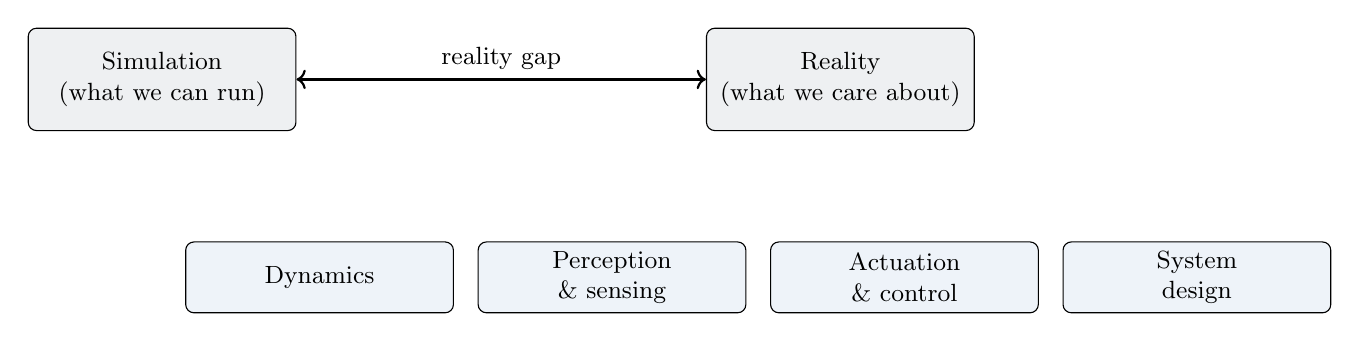
\begin{tikzpicture}[node distance=1.2cm, every node/.style={font=\small},
 box/.style={draw, rounded corners=3pt, minimum width=3.4cm, minimum height=0.9cm, align=center, fill=cblue!8},
 big/.style={draw, rounded corners=3pt, minimum width=3.4cm, minimum height=1.3cm, align=center, fill=cgray!12}]
\node[big] (sim) {Simulation\\(what we can run)};
\node[big, right=5.2cm of sim] (real) {Reality\\(what we care about)};
\draw[<->, thick] (sim) -- node[above]{reality gap} (real);
\node[box, below=1.4cm of sim, xshift=2.0cm] (a) {Dynamics};
\node[box, right=0.3cm of a] (b) {Perception\\\& sensing};
\node[box, right=0.3cm of b] (c) {Actuation\\\& control};
\node[box, right=0.3cm of c] (d) {System\\design};
\end{tikzpicture}
\caption{The gap is not one number. The paper (Fig.~1) splits it into four families.}
\end{figure}

% ============================================================ 2
\section{Words you need first}

\begin{description}[leftmargin=1.2cm,labelwidth=1cm,itemsep=3pt]
\item[Simulation] A computer program that imitates the physics of a robot and its environment.
In this paper it also includes imitating the \emph{sensors} (cameras, encoders).
\item[Reality gap] The difference between the simulated and the real environment.
\item[Sim-to-real transfer] Taking something developed in simulation (a trained controller,
a tuned estimator, a design) and running it in the real world.
\item[Real-to-sim] The opposite direction: using real data to \emph{improve} the simulator
(for example, measuring the real friction and putting it into the simulator).
\item[Policy $\pi$] The decision rule of the robot: it takes what the robot knows and outputs
an action. A neural network, a planner or a controller can all be seen as a policy.
\item[State $s$] Everything that is true about the world at one moment (ball position and
velocity, arm joint angles, the real friction value\ldots). Usually the robot \emph{cannot}
see all of it.
\item[Observation $z$] What the sensors actually deliver (a depth image, a noisy 3D point).
\item[Belief $b$] A probability distribution over states that the robot keeps because it cannot
see the state exactly. A Kalman filter's mean and covariance are exactly a (Gaussian) belief.
\item[Dynamics] The rule that tells how the state changes from one time step to the next.
\item[Divergence $D$] A number that measures how different two probability distributions are
(zero if identical). KL divergence is the most common one.
\item[System identification] Measuring unknown physical parameters (friction, mass) from real
data and putting them into the model.
\item[Domain randomization] Training or testing across many randomly different simulated
worlds so that the robot does not depend on one exact version of the simulator.
\item[Privileged information] Information that exists in simulation but not in reality, for
example the exact ball position without any sensor.
\item[Success rate] Number of successful trials divided by number of trials.
\end{description}

% ============================================================ 3
\section{Section 1 of the paper: why simulation, and why it is hard}

\subsection{The benefits the authors list \textnormal{\textbf{(paper)}}}
\begin{itemize}
\item \textbf{Scalability, safety, efficiency.} A robot can be trained in simulation before it
touches the real world.
\item \textbf{Benchmarking.} Algorithms can be compared over many simulated scenarios, with
repeatable results; this is ``impossible in real-world robotics systems due to their stochastic
nature''.
\item \textbf{Data generation.} Many robots can run faster than real time and in parallel.
\item \textbf{Real-world bottlenecks.} Real data collection is limited by hardware cost, human
dependence, and difficulty of automation.
\end{itemize}

The authors compare with other fields: progress in language and vision depended on huge
\emph{datasets}. Robotics lacks that because static datasets cannot capture an \emph{interactive}
world (the data depend on what the robot does). Simulation is the proposed substitute.

\subsection{The problem \textnormal{\textbf{(paper)}}}
\begin{itemize}
\item ``There are no perfect simulators, and therefore there is always a difference from the
real world, which we call reality gap.''
\item It is a common misconception to treat the gap as \emph{one thing}; it is a large number
of \emph{sub-gaps}, one for each physical mechanism the simulator fails to copy.
\item A policy can score very well in simulation \emph{because it exploits simulator errors and
corner cases}. In the real world this is useless and can even be dangerous to the robot, its
surroundings and people nearby.
\end{itemize}

\begin{toy}[Toy example: a policy that exploits the simulator]
Suppose our simulator lets the ball pass \emph{through} a wall corner when the speed exceeds
$3$ m/s because of a bug in the collision code. A catching policy trained there may learn
``wait at the corner; the ball always comes out there''. It scores $100\%$ in simulation and
$0\%$ in reality. The policy did not learn catching; it learned the bug.
\end{toy}

\subsection{What has worked anyway \textnormal{\textbf{(paper)}}}
The survey notes that sim-to-real has still produced strong results: quadruped and biped
locomotion, agile quadrotor flight (including champion-level drone racing), and manipulation such
as table-top rearrangement and assembly. Modern simulators run on GPUs and simulate thousands of
robots at once. Open difficulties named in the introduction are photorealistic rendering (more
generally, \emph{sensor modeling}) and simulation of contacts, deformations and material
variations. Notice that the first is exactly the part of the paper that matters most for our
chapter.

\subsection{Roadmap of the paper \textnormal{\textbf{(paper)}}}
Section 2: formal problem. Section 3: causes of the gap. Section 4: solutions. Section 5:
metrics. Section 6: open problems and outlook.

% ============================================================ 4
\section{Section 2 of the paper: the mathematics, step by step}

This is the only mathematical part of the paper, but everything later depends on it. I go slowly.

\subsection{The robot problem as a POMDP \textnormal{(paper Sec.~2.1)}}

A \textbf{POMDP} (Partially Observable Markov Decision Process) is the standard mathematical
model of an agent that acts in a world it cannot fully see. The paper defines it as a
seven-element tuple:
\begin{eqbox}[POMDP tuple (paper, Sec.~2.1)]
\[
M=(\mathcal S,\mathcal A,T,R,\mathcal Z,O,\gamma)
\]
\end{eqbox}

\begin{center}
\renewcommand{\arraystretch}{1.25}
\begin{tabularx}{\textwidth}{@{}l X X@{}}
\toprule
Symbol & Meaning & For the catching robot \\
\midrule
$\mathcal S\subseteq\mathbb R^n$ & state space: all possible configurations of robot and world &
ball position and velocity, arm joint angles, floor friction \\
$\mathcal A\subseteq\mathbb R^m$ & action space: all commands the robot can send &
joint torques or velocity commands, gripper command \\
$T:\mathcal S\times\mathcal A\to\mathcal S$ & transition dynamics: how the state evolves given
the action & physics of the ball sliding, bouncing, being hit \\
$R:\mathcal S\times\mathcal A\to\mathbb R$ & reward: how good the situation is &
$+1$ if the ball is caught \\
$\mathcal Z\subseteq\mathbb R^h$ & observation space: everything the sensors can output &
depth images, joint encoder readings \\
$O:\mathcal S\to\mathcal Z$ & sensor model: maps the hidden state to an observation $z_t$ &
camera + detector: ball state $\to$ noisy 3D point \\
$\gamma\in[0,1)$ & discount factor: weight of future versus immediate reward &
close to $1$ means ``the final catch matters most'' \\
\bottomrule
\end{tabularx}
\end{center}

The word \emph{partially observable} means: the robot never sees $s_t$, only $z_t=O(s_t)$. To act
sensibly it keeps a \textbf{belief} $b_t\in\mathcal B(\mathcal S)$, a probability distribution
over states, updated from the history of past actions and observations. The goal is to find a
policy $\pi:\mathcal B(\mathcal S)\to\mathcal A$ (``given my belief, choose an action'') that
maximises the expected discounted return:
\begin{eqbox}[Objective (paper, Eq.~1)]
\[
\pi^{*}=\arg\max_{\pi}\ \mathbb E\Big[\sum_{t=0}^{\infty}\gamma^{t}\,R\big(s_t,\pi(b_t)\big)\Big]
\]
\end{eqbox}
Read it from the inside out: at each time $t$ the robot is in state $s_t$, uses its belief $b_t$
to pick the action $\pi(b_t)$, and receives the reward $R$. Multiplying by $\gamma^t$ makes later
rewards count less. The sum adds everything up, the expectation $\mathbb E$ averages over the
randomness, and $\arg\max$ picks the best policy.

\begin{idea}[Why this matters for us]
In the paper, ``belief'' is just one line. In our chapter it is the \emph{whole subject}. A
Kalman filter, an EKF, KalmanNet or a transformer predictor are all different ways to compute
the belief $b_t$ (at least a mean and a covariance) from the observations $z_{1:t}$. Our
chapter-1 planners were written for the case ``MDP'': they read the true state $s_t$ directly.
Chapter 2 turns them into the POMDP case.
\end{idea}

The paper adds a footnote: when sensors give the full state without noise (simulation with
privileged information), observations equal states and the POMDP collapses to an ordinary MDP.
The paper says in practice $b_t$ is often replaced by a compact feature vector extracted from raw
observations such as camera images.

\begin{figure}[H]
\centering
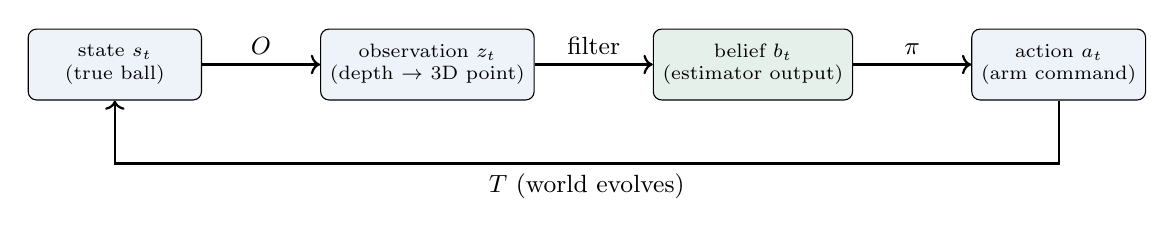
\begin{tikzpicture}[font=\small, node distance=1.5cm,
 b/.style={draw, rounded corners=3pt, minimum height=0.9cm, minimum width=2.2cm, align=center, fill=cblue!8, font=\scriptsize}]
\node[b] (s) {state $s_t$\\(true ball)};
\node[b, right=of s] (z) {observation $z_t$\\(depth $\to$ 3D point)};
\node[b, right=of z, fill=cgreen!12] (bel) {belief $b_t$\\(estimator output)};
\node[b, right=of bel] (a) {action $a_t$\\(arm command)};
\draw[->, thick] (s) -- node[above]{$O$} (z);
\draw[->, thick] (z) -- node[above]{filter} (bel);
\draw[->, thick] (bel) -- node[above]{$\pi$} (a);
\draw[->, thick] (a.south) -- ++(0,-0.8) -| node[pos=0.25,below]{$T$ (world evolves)} (s.south);
\end{tikzpicture}
\caption{The POMDP loop for the catching robot. Chapter 2 builds the green box.}
\end{figure}

\subsection{A simulation is an approximation \textnormal{(paper Sec.~2.2)}}

Let $T_r(s_{t+1}\mid s_t,a_t)$ be the \emph{real} dynamics (the unknowable perfect description of
how the world evolves) and $O_r(z_t\mid s_t)$ the \emph{real} observation model. A simulation uses
physical models from first principles, numerical integration and simplifications to reduce cost:
\[
T_s(s_{t+1}\mid s_t,a_t)\approx T_r(s_{t+1}\mid s_t,a_t),\qquad
O_s(z_t\mid s_t)\approx O_r(z_t\mid s_t)\quad \forall s_t\in\mathcal S,\ a_t\in\mathcal A.
\]
Note that the paper writes $T$ and $O$ as \emph{conditional probability distributions} here (the
vertical bar), although Sec.~2.1 introduced them as functions. That is the usual way: a
function is the special case of a distribution with no randomness. \textbf{(paper)} states that
``perfect fidelity is impractical and computationally infeasible'' because of the inherent
complexity of friction, noise, sensor latency and so on.

\subsection{The reality gap and the performance gap \textnormal{(paper Sec.~2.3)}}

\begin{eqbox}[Definitions (paper, Eq.~2)]
\begin{align*}
G_{\mathrm{dyn}}(\Ms,\Mr)&=\mathbb E_{(s,a)\sim \Mr}\Big[D\big(\Tsim(\cdot\mid s,a)\,\big\|\,\Treal(\cdot\mid s,a)\big)\Big]\\
G_{\mathrm{perc}}(\Ms,\Mr)&=\mathbb E_{s\sim S_r}\Big[D\big(\Osim(\cdot\mid s)\,\big\|\,\Oreal(\cdot\mid s)\big)\Big]
\end{align*}
\end{eqbox}

How to read $G_{\mathrm{dyn}}$: go to the \emph{real} world, look at the states and actions $(s,a)$
that really occur. For each of them ask the simulator and the real world ``where does the state go
next?'' Each answers with a probability distribution; $D$ measures how different the two answers
are. Average over all situations. If the simulated dynamics were perfect, every $D$ would be zero.
$G_{\mathrm{perc}}$ is the same idea for the \emph{sensor}: ``given this true state, how does the
simulated sensor output distribution differ from the real one?''

\begin{toy}[Toy example: measuring a perception gap by hand]
Take one single true state: the ball is exactly $2.000$ m from the camera. Suppose the depth
reading in the \emph{real} camera is Gaussian with standard deviation $5$ mm, and in the
\emph{simulator} we used a nearly noise-free camera with $0.5$ mm. For two Gaussians with the same
mean, $\mathrm{KL}(N(0,\sigma_1^2)\,\|\,N(0,\sigma_2^2))=\ln(\sigma_2/\sigma_1)+\sigma_1^2/(2\sigma_2^2)-\tfrac12$.
\begin{itemize}
\item $D=\mathrm{KL}(\text{sim}\,\|\,\text{real})=\ln 10+0.25/50-0.5\approx 1.81$ nats.
\item $D=\mathrm{KL}(\text{real}\,\|\,\text{sim})=\ln 0.1+25/0.5-0.5\approx 47.2$ nats.
\end{itemize}
Two lessons. (i) Which divergence and which \emph{direction} you choose changes the number by a
factor of $26$. (ii) A simulator that is \emph{too clean} is punished hard when compared in the
second direction; with zero noise the second value becomes infinite.
\end{toy}

The \textbf{performance gap} is a different object. It does not compare worlds; it compares the
\emph{score of one fixed policy} in the two worlds. Let $\tau=(s_0,z_0,a_0,s_1,z_1,a_1,\dots,s_T,z_T)$
be one closed-loop trajectory. The expected return of policy $\pi$ in a world $M$ is
\begin{eqbox}[Return and performance gap (paper, Eqs.~3 and 4)]
\[
J_M(\pi)=\mathbb E_{\tau\sim p(\tau\mid\pi,M)}\Big[\sum_{t=0}^{T}\gamma^{t}R\big(s_t,\pi(b_t)\big)\Big],\qquad
G_{\mathrm{perf}}(\Ms,\Mr,\pi)=\big|J_{\Ms}(\pi)-J_{\Mr}(\pi)\big|
\]
\end{eqbox}
In words: run the same policy in simulation and in reality, compute the average score in each, and
take the absolute difference. The final objective (paper, Eq.~5) is to find the policy that
\emph{minimises} this gap (the paper writes ``$\min$'' where the correct symbol would be
$\arg\min$).

\begin{idea}[The most important sentence of Section 2]
\textbf{(paper)}: removing $G_{\mathrm{dyn}}$ and the perception gap completely is neither
practically achievable nor required. Transfer can succeed if the policy is \emph{robust} to the
differences. In other words: what matters for the task is $G_{\mathrm{perf}}$, not the size of the
physical gap. A big gap in something your task never touches costs you nothing.
\end{idea}

\begin{warn}[My critical comments on Section 2]
\begin{itemize}
\item The divergence $D$ is left unspecified (KL? Wasserstein? total variation?) and so is its
\emph{direction}. As my toy example shows, this matters numerically. The definitions are therefore
conceptual, not directly computable recipes.
\item The paper writes $G_{\mathrm{obs}}$ once in the text after defining $G_{\mathrm{perc}}$; this is
a notation slip for the same quantity.
\item $G_{\mathrm{perc}}$ requires samples from the \emph{real} sensor. In a simulation-only project
like ours, $O_r$ is unavailable. We can only make $O_s$ \emph{plausible} using literature, not
measure the gap.
\end{itemize}
\end{warn}

% ============================================================ 5
\section{Section 3 of the paper: where the gap comes from}

This is the largest section. The paper walks through four families, each with a list of concrete
mechanisms, and attaches a short ``\textbf{Symptom}'' to many of them (what goes wrong in a robot
that ignores the mechanism). I repeat the lists in my own words and add where each item touches
our project.

\subsection{Dynamics \textnormal{(paper Sec.~3.1)} \textnormal{(the transition model $T$)}}
\textbf{(paper)} calls dynamics ``one of the most important causes of the reality gap''. When a
simulator is built, many decisions are made about what to include, which parameters to use, and
how to represent continuous phenomena in discrete computations. A policy trained in inaccurate
dynamics may learn to \emph{exploit} the inaccuracies.

\subsubsection*{3.1.1 Modeling}
\begin{itemize}
\item \textbf{Rigid-body dynamics.} Simulators usually assume perfectly rigid bodies and ideal
joints, but real links bend and vibrate under load, joints have damping, internal springs and
backlash. \emph{Symptom:} a policy trained with rigid-body assumptions behaves unexpectedly with
real deformable objects.
\item \textbf{Chaotic nature.} Some phenomena (turbulence, fluid flow) depend so sensitively on
initial conditions that they are non-reproducible even with a perfect model. \emph{Symptom:} an
over-fitted policy with slightly different initial conditions may fail unpredictably.
\item \textbf{Stochasticity.} Ground robots meet random surface and friction variations and
debris. Simulators either ignore this or use simple Gaussian noise and miss complex space-time
correlations and non-linear couplings.
\item \textbf{Battery.} Motor torque scales with voltage; voltage drops with load, temperature and
age, so rapid accelerations may suffer a torque deficit absent in simulation. \emph{Symptom:}
unmodeled battery dynamics make the policy produce less torque than needed.
\item \textbf{Contact dynamics.} Real contact is nonlinear: materials deform, friction varies with
relative velocity, contact switches between sticking, slipping and separation. Simulators use
simplified models (point contacts, linearised friction cones, spring-damper contact), which can
create spurious forces and unstable grasps. \emph{Symptom:} a policy may fail to grasp because its
model of contact is simplistic.
\end{itemize}

\begin{ours}[Our chapter: what this means for the ball]
Our ball hits walls (contact), slides with friction that may vary (stochasticity and
parameterisation), and may be fast. MuJoCo handles contact with a soft contact model; we must
\textbf{not} assume its bounce equals a perfect restitution law. This is why papers 05, 19 and 01
(bounce and wall models learned from data) are in the chapter.
\end{ours}

\subsubsection*{3.1.2 Parameterization}
Even when the right physical \emph{model} is used, the \emph{numbers} (friction, aerodynamics,
mass, inertia) are hard to measure and can change over time. \emph{Symptom:} the policy overshoots
or undershoots because its learned dynamics are based on wrong parameters.

\subsubsection*{3.1.3 Numerical integrators}
The simulator turns differential equations into steps (Euler, Runge--Kutta, etc.). Smaller steps
or higher-order methods are more accurate but cost computation. \emph{Symptom:} small integration
errors accumulate and performance degrades over long tasks.

\begin{toy}[Toy example: integrator error on a sliding ball]
A ball decelerates with $a=-0.5$ m/s$^2$ from $v_0=3$ m/s. The exact stopping distance is
$v_0^2/(2|a|)=9$ m. With a crude explicit Euler step of $0.5$ s (position advanced with the old velocity, then
velocity updated) the simulated ball travels $9.75$ m. A $5$ ms step gives $9.0075$ m. The
physics did not change; only the integrator did. (Numbers invented, computed by hand.)
\end{toy}

\subsubsection*{3.1.4 Human--robot interaction}
Humans are simulated as simple agents with predefined motion. \emph{Symptom:} a policy exploits
wrong assumptions about human behaviour. (Not relevant for our ball.)

\subsubsection*{3.1.5 Unmodeled effects}
Wear and tear (backlash, stiffness changes) and thermal effects (temperature changes motors,
sensors, batteries). \emph{Symptom:} performance drifts over time or vibrations appear.

\subsubsection*{3.1.6 Asset fidelity}
The environment is represented by digital assets: geometry (primitives, meshes, signed distance
fields) and \emph{material parameters such as friction coefficients, restitution and density}.
For speed, these are simplified. \emph{Symptom:} the policy acts on inaccurate geometry and
collides with unmodeled effects.

\begin{ours}[Our chapter]
The words ``friction coefficient'' and ``restitution'' are exactly the numbers of our walls and
floor. In MuJoCo they are set by hand. Our estimator will be tested against \emph{several
values} of them, not one.
\end{ours}

% ------------------------------------------------------------
\subsection{Perception and sensing \textnormal{(paper Sec.~3.2)} \textnormal{(the observation model $O$)}}
This is the subsection that matters most for us. The gap is defined as differences in the
observation model $O$. The paper observes that advanced renderers have improved the realism of
sensors, but they ``still fall short of capturing the full complexity and variability of the real
world''.

\subsubsection*{3.2.1 Sensor model}
Simulated sensors are designed to mimic field of view, resolution and noise patterns, how they
respond to motion, and how they are mounted. Per sensor type \textbf{(paper)}:
\begin{itemize}
\item \textbf{RGB cameras.} Isaac Sim uses ray tracing and physically based rendering. CARLA and
AirSim (Unreal Engine) simulate realistic visuals. Simulators optimised for real-time speed, such
as Gazebo Classic and early MuJoCo, use simplified OpenGL rendering with idealised pinhole
cameras and Z-buffer depth; they omit lens flares, chromatic aberration, flying pixels and rolling
shutter distortion.
\item \textbf{Depth sensors.} Stereo, structured light (Kinect v1) and time of flight (RealSense)
can be simulated. Synthetic depth maps come from rendered 3D geometry and ``typically assume
ideal depth projections and often omit real-world artifacts such as quantization noise, depth
shadows, and ambient light interference''.
\item \textbf{LiDAR.} Ray casting from the sensor origin; beam divergence, reflectivity, and
angle-of-incidence effects are hard to reproduce.
\item \textbf{Other sensors.} Joint encoders, IMUs, GPS, tactile: often idealised, ignoring IMU
drift, GPS multipath and \emph{latency}.
\end{itemize}
\emph{Symptom (paper):} sensor-specific artifacts can lead to massive sim-to-real discrepancies
in the distribution of observations.

\subsubsection*{3.2.2 Sensor noise}
Real measurements are noisy because of thermal effects, quantization and environmental
interference. Crucially, the paper says noise is often \textbf{non-Gaussian, state-dependent,
temporally correlated} and influenced by motion, temperature, lighting and surface properties.
For depth sensors specifically: ``range-dependent uncertainty, structured missing data at depth
discontinuities, and surface-dependent noise patterns''. Yet ``many simulators use simple Gaussian
noise models with fixed variance''. \emph{Symptom:} policies trained on simple Gaussian noise may
overfit and fail under complex, state-dependent, temporally correlated real noise.

\begin{toy}[Toy example: why ``fixed variance'' is wrong for depth]
A fixed-variance simulator says: depth error is always $\pm 5$ mm. A real range sensor behaves more
like: error $\pm 2$ mm at $1$ m but $\pm 18$ mm at $3$ m (error grows with distance, as paper 12
will explain later). A tracker tuned for $\pm5$ mm will trust the far-away ball too much and
under-trust the near one. Numbers invented; the \emph{shape} (error grows with range) is what the
survey states.
\end{toy}

\subsubsection*{3.2.3 Environment representation}
Low-resolution assets, generic materials, missing HDRI backgrounds, and failing to distinguish
static from dynamic bodies (which \emph{obscures motion and occlusion relationships}) degrade
perceptual realism. \emph{Symptom:} the robot fails to recognise objects or gets lost in a real
room that looks different from the visually simple simulation.

\subsubsection*{3.2.4 Robot model}
Robot models from CAD/URDF/USD files are structurally accurate but omit manufacturing
tolerances, wear and backlash, leading to self-collisions or unstable motion.

\subsubsection*{3.2.5 Collision sensing}
Collision detection is simplified (bounding volumes, convex decompositions, sphere
decompositions) and evaluated at discrete time steps, limiting accuracy for fine contact.

\begin{ours}[Our chapter: the perception checklist]
Combining 3.2.1--3.2.3 gives a practical \textbf{checklist for our simulated depth camera}
(Step 2 of the chapter): (1) range-dependent depth noise; (2) quantisation of depth values;
(3) \emph{missing} depth at edges and on small objects (dropout); (4) latency; (5) occlusion
by walls or the arm; (6) a detector that can fail. The survey states these effects exist; it does
\textbf{not} give numbers. The numbers come later from papers 12 (depth noise law) and 11
(tracking loss and delay).
\end{ours}

% ------------------------------------------------------------
\subsection{Actuation and control \textnormal{(paper Sec.~3.3)}}
Actuators and their low-level control loops are ``the last interface of the robot's actions and
the real world''. Even with perfect perception and dynamics, a mismatch here can dominate
behaviour.
\begin{itemize}
\item \textbf{Actuator models.} Simulators treat motors as ideal, instantaneous, linear
(first-order); real actuators have electrical and mechanical time constants, phase lag,
dead-zones, backlash, slew-rate limits and hysteresis.
\item \textbf{Low-level control.} Policies rarely send raw torque; vendor firmware and hidden
filters (anti-aliasing, resonance suppression, saturation, anti-windup, rate limits) modify
commands. Simulators do not model them. \emph{Symptom:} commands do not produce the expected
motion.
\item \textbf{Power electronics.} Drivers and inverters add latency of hundreds of microseconds,
PWM quantisation and dead zones near zero crossing, and hard current/voltage caps. \emph{Symptom:}
fine motion fails with jitter or dead zones near zero velocity.
\end{itemize}
For our Panda this is the \emph{chapter-1} territory (the MPC and TOPP-RA stack). Chapter 2 does
not touch it.

% ------------------------------------------------------------
\subsection{System design \textnormal{(paper Sec.~3.4)}}
\begin{itemize}
\item \textbf{Communication.} Real systems have delays and packet loss, simulation almost none.
\emph{Symptom:} delays cause freezing, slowdown or jerky fallback motion.
\item \textbf{Safety mechanisms.} Virtual walls, limits and safe-stop behaviours exist on real
robots, not in simulation.
\item \textbf{POMDP formulation.} ``Simulated POMDPs often feature unrealistic information and
behaviors''. Rewards and termination may use privileged data (exact collisions) unavailable in
reality; environment resets may place objects at exact positions with preset velocities, which is
impossible in reality, so state--action distributions differ.
\item \textbf{Implementation details.} Continuous processes are discretised; control loops can
run at different frequencies in simulation and reality. \emph{Symptom:} instability from
mismatched control frequencies or numerical methods.
\end{itemize}

\begin{ours}[Our chapter: we have exactly this problem]
Chapter 1 gave the planners the \emph{exact} ball position and velocity (privileged information)
and launched the ball with exact preset velocity. The survey names both as sources of a gap.
Chapter 2 removes the first (estimated state instead of true state). The second one (exact
resets) is unavoidable in simulation, but we can \emph{randomise} the launch states widely so the
evaluation covers many situations.
\end{ours}

\begin{figure}[H]
\centering
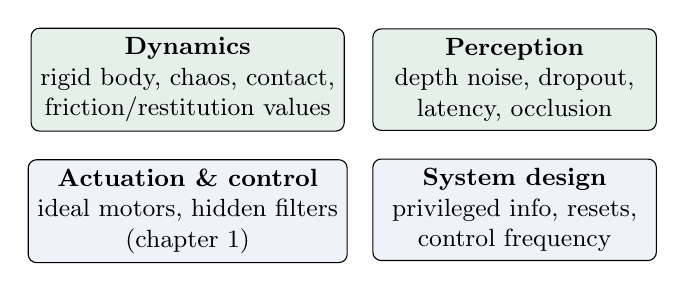
\begin{tikzpicture}[font=\small, node distance=0.35cm,
 f/.style={draw, rounded corners=3pt, minimum width=3.6cm, minimum height=1.0cm, align=center, fill=cblue!8}]
\node[f, fill=cgreen!12] (a) {\textbf{Dynamics}\\rigid body, chaos, contact,\\friction/restitution values};
\node[f, fill=cgreen!12, right=of a] (b) {\textbf{Perception}\\depth noise, dropout,\\latency, occlusion};
\node[f, below=of a] (c) {\textbf{Actuation \& control}\\ideal motors, hidden filters\\(chapter 1)};
\node[f, below=of b] (d) {\textbf{System design}\\privileged info, resets,\\control frequency};
\end{tikzpicture}
\caption{The four families. Green = the two that our estimator comparison touches directly.}
\end{figure}

% ============================================================ 6
\section{Section 4 of the paper: what to do about it}

\textbf{(paper)} first gives a six-step ``recipe'':
\begin{enumerate}
\item Design a simulation that represents all variables relevant for the target application.
\item Reduce the different components of the reality gap as much as possible.
\item Design training methods that help overcome the remaining gap.
\item Train policies in simulation (ideally massively parallel).
\item Evaluate policies in the target real-world environment.
\item Adjust simulation parameters from real performance and retrain.
\end{enumerate}
Then two big families (Fig.~3 of the paper):
\begin{itemize}
\item \textbf{Reducing the gap}: remove sources of the gap by making the simulation or the system
better.
\item \textbf{Overcoming the gap}: assume a fixed remaining gap and make the robot software
agnostic, adaptive or passive to what cannot be modelled.
\end{itemize}

\begin{figure}[H]
\centering
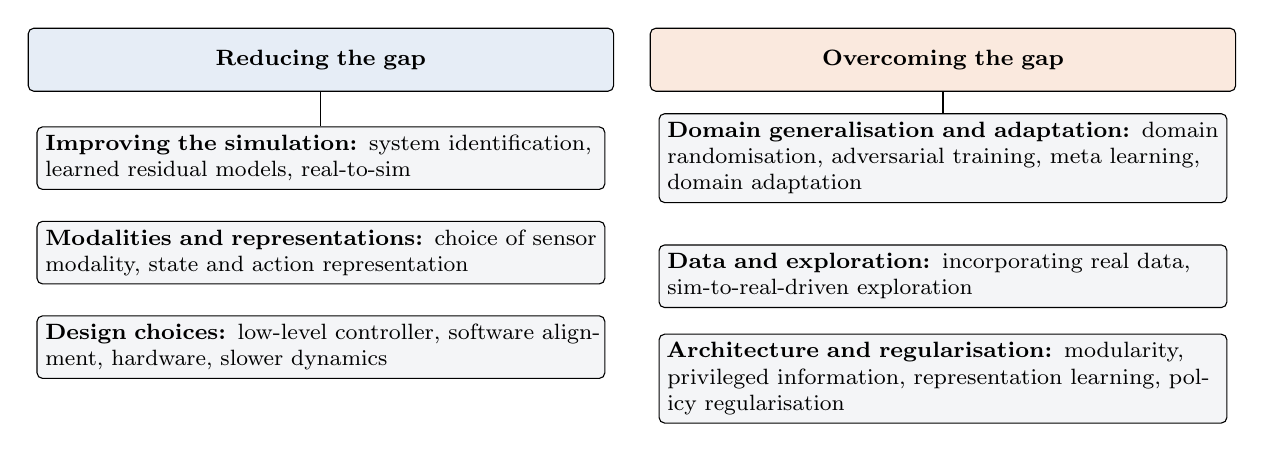
\begin{tikzpicture}[font=\footnotesize,
 t/.style={draw, rounded corners=2pt, align=center, minimum height=0.8cm, text width=7.2cm, fill=cblue!12},
 u/.style={draw, rounded corners=2pt, align=center, minimum height=0.8cm, text width=7.2cm, fill=corange!15},
 n/.style={draw, rounded corners=2pt, align=left, text width=7.0cm, fill=cgray!8, inner sep=3pt}]
\node[t] (red) at (0,0) {\textbf{Reducing the gap}};
\node[n] (r1) at (0,-1.25) {\textbf{Improving the simulation:} system identification, learned residual models, real-to-sim};
\node[n] (r2) at (0,-2.45) {\textbf{Modalities and representations:} choice of sensor modality, state and action representation};
\node[n] (r3) at (0,-3.65) {\textbf{Design choices:} low-level controller, software alignment, hardware, slower dynamics};
\node[u] (ov) at (7.9,0) {\textbf{Overcoming the gap}};
\node[n] (o1) at (7.9,-1.25) {\textbf{Domain generalisation and adaptation:} domain randomisation, adversarial training, meta learning, domain adaptation};
\node[n] (o2) at (7.9,-2.75) {\textbf{Data and exploration:} incorporating real data, sim-to-real-driven exploration};
\node[n] (o3) at (7.9,-4.05) {\textbf{Architecture and regularisation:} modularity, privileged information, representation learning, policy regularisation};
\draw (red) -- (r1); \draw (ov) -- (o1);
\end{tikzpicture}
\caption{Taxonomy of solutions (my redrawing of the paper's Fig.~3).}
\end{figure}

\subsection{Reducing the gap \textnormal{(paper Sec.~4.1)}}

\subsubsection*{4.1.1 Improving the simulation}
\begin{itemize}
\item \textbf{System identification.} Repeatedly shown to be crucial in navigation, locomotion and
manipulation. A recent trend is \emph{online, iterative} identification with data from successive
real evaluations. Besides physical parameters, one should identify system-level parameters such as
\textbf{latency, control frequency and actuation delay}.
\item \textbf{Learned residual models.} If the simulator's model is fundamentally wrong (rigid
bodies for a compliant object), identifying parameters will not help. Instead \emph{learn a
model that corrects the simulator}, so the combined model matches reality. The paper gives
examples: an LSTM trained on the differences between simulated and real trajectories (Golemo et
al.); a stochastic RNN added to a deterministic simulator for contact uncertainty (Ajay et al.);
a network added to an analytical model for compliance and friction (Gruenstein et al.); a network
adding residual forces to a blade-element aerodynamic model for fast quadrotor flight (Bauersfeld
et al.); corrective forces on a finite-element soft arm (Gao et al.). Others instead learn a
mapping that \emph{corrects the action} (Christiano et al., Hanna et al.).
\item \textbf{Real-to-sim first.} Use real data to build accurate geometry (3D reconstruction),
kinematics and dynamics (articulation from video) and visuals (novel-view synthesis).
\end{itemize}

\begin{ours}[Our chapter]
Residual learning is the idea behind our learned estimators: a physics model (constant velocity
plus friction plus wall bounce) as the backbone, and a small learned correction
(KalmanNet's learned gain, differentiable-EKF's learned Q and R, papers 04, 06). System
identification of friction and restitution is paper 19's Bayesian-optimisation step.
\end{ours}

\subsubsection*{4.1.2 Choice of modalities and representations}
\begin{itemize}
\item \textbf{Modalities.} Depth observations or point clouds give a \emph{smaller} reality gap
than RGB images, ``a common practice in the field'', because RGB images are hard to render
photo-realistically and contain features that are very complex to model.
\item \textbf{State representations.} Keypoint detections, visual feature tracking and foundation
model embeddings are good abstractions that reduce the sensory gap.
\item \textbf{Action representations.} For manipulation, joint-velocity control spaces transfer
better than torque.
\end{itemize}
This supports our earlier decision to use a depth camera rather than an RGB-only pipeline.

\subsubsection*{4.1.3 Design choices}
\begin{itemize}
\item \textbf{Low-level controller improvements.} Higher control frequency or bandwidth helps the
system respond to discrepancies (e.g.\ high-frequency impedance controllers).
\item \textbf{Software-stack alignment.} Match control rates, filters and safety checks between
simulation and the real robot.
\item \textbf{Hardware design.} Low-latency actuators and sensors with well-characterised noise make
simulation easier and reduce the need for complex identification.
\item \textbf{Constraining system dynamics.} Operating at \emph{lower speeds} or avoiding aggressive
maneuvers makes the system less sensitive to model inaccuracies, delays and perception noise
(quasi-static regimes transfer more reliably).
\end{itemize}

\begin{ours}[Important consequence of the last bullet]
The survey says: \emph{slow motion shrinks the gap}. Our chapter deliberately allows
\textbf{fast balls with varying velocities and accelerations}. By the survey's own logic this makes
our problem \emph{more sensitive} to delay and noise. A 40 ms delay costs $2$ cm at $0.5$ m/s but
$20$ cm at $5$ m/s. So we should expect (and report) that the ranking of estimators changes with
ball speed.
\end{ours}

\subsection{Overcoming the gap \textnormal{(paper Sec.~4.2)}}

\subsubsection*{4.2.1 Domain generalisation and adaptation}
\begin{itemize}
\item \textbf{Domain randomization (DR).} Train over a broad distribution of simulated worlds:
visual parameters (texture, lighting), observation and action noise, physics (mass, inertia),
\textbf{system delays}, object properties. The robot then learns behaviour valid for all of them,
including the real one. DR reduces the need for painstaking system identification. Earliest use:
drone navigation; since then dexterous manipulation, quadruped locomotion and champion-level drone
racing. Extensions: \emph{automatic DR} that widens ranges as the policy improves (Akkaya et al.),
estimating DR ranges from an offline real dataset (Tiboni et al.), and using real data to infer
simulation parameters (Chebotar et al.).
\item \textbf{Adversarial training.} Train an adversary that applies disturbances to destabilise
the main agent (Pinto et al.).
\item \textbf{Meta learning.} Train over a distribution of simulation parameters so the policy can
internally recognise the variation; rapid motor adaptation (RMA) learns an encoder of environment
dynamics from privileged information in simulation.
\item \textbf{Domain adaptation.} Make the policy robust to the distribution shift in
\emph{observations}.
\end{itemize}

\begin{toy}[Toy example: domain randomization for our estimator]
Instead of testing a tracker with one setup (depth noise $5$ mm, delay $40$ ms, friction $0.3$),
we draw each episode's values: noise $\sim U(1,10)$ mm, delay $\sim U(10,80)$ ms, friction
$\sim U(0.1,0.5)$, dropout $\sim U(0,30)\%$. An estimator that scores well across the whole cloud
is robust; one that is great only at the centre is fragile. (Ranges invented.)
\end{toy}

\subsubsection*{4.2.2 Data selection and exploration}
Use real data to inform simulation training (e.g.\ penalise learning from simulated state--action
pairs that differ from real dynamics; co-train with real and simulated data), and explore in ways
that expose the policy to transfer-relevant interactions (e.g.\ run exploration policies in the
real world to identify critical parameters).

\subsubsection*{4.2.3 Policy architecture and regularisation}
\begin{itemize}
\item \textbf{Modularity.} Split vision, policy and low-level control into independent modules; this
makes transfer more robust (examples in pushing and driving).
\item \textbf{Privileged information.} Information available in simulation but not reality can
speed up learning: RMA's latent encoder; asymmetric actor--critic (critic sees privileged state,
actor sees real observations); teacher--student distillation (teacher with privileged state,
student with real observations).
\item \textbf{Representation learning.} Self-supervised losses that make features robust to domain
shift (aligning sim and real feature distributions, adversarial encoder adaptation, contrastive
learning to ignore background).
\item \textbf{Policy regularisation.} Penalise action magnitude or consecutive action differences,
or use smoothness losses to keep behaviour gentle.
\end{itemize}

\begin{ours}[Our chapter: privileged information is a training tool, not only a defect]
In our simulator the \textbf{true ball state is available for free}. That is privileged information
in the survey's sense. We will use it twice: (i) \emph{as the label} to train the learned
estimators (KalmanNet, differentiable EKF, NODE filter, sequence predictor) and (ii) \emph{as the
reference} to compute estimation error. At deployment (and at evaluation of catch success) the
planner may only see the \emph{estimate}. Keeping those two roles separate is the whole
discipline of the chapter.
\end{ours}

% ============================================================ 7
\section{Section 5 of the paper: metrics}

The paper distinguishes metrics that evaluate the \emph{gap itself} from metrics that evaluate
\emph{transfer performance}.

\subsection{Assessing the reality gap \textnormal{(paper Sec.~5.1)}}

\subsubsection*{Sim-to-real Correlation Coefficient (SRCC)}
\begin{eqbox}[SRCC (paper, Eq.~6; proposed by Kadian et al.)]
\[
\mathrm{SRCC}=\frac{\sum_{i=1}^{N}(x_i-\bar x)(y_i-\bar y)}
{\sqrt{\sum_{i=1}^{N}(x_i-\bar x)^2}\ \sqrt{\sum_{i=1}^{N}(y_i-\bar y)^2}}
\]
\end{eqbox}
$x_i$ is the performance (e.g.\ success rate) of the $i$-th policy in simulation, $y_i$ in the real
world; $\bar x,\bar y$ are the means. This is the ordinary Pearson correlation. Close to $+1$: the
simulator ranks policies the way reality does, so improvements in simulation will really help.
Near $0$: simulation says little about reality. The authors stress that a simulator with high
average real performance but low SRCC is still a problem, because you can no longer trust
simulation to choose between designs.

\begin{toy}[Toy example: SRCC by hand]
Four estimators evaluated in simulation: success $x=(50,60,80,90)\,\%$; mean $\bar x=70$.
\emph{Case A} (real world gives $y=(20,30,50,60)\,\%$, mean $40$): the deviations of $y$ are exactly
those of $x$, so SRCC $=1.00$. The simulator is pessimistic in absolute terms but ranks perfectly.
\emph{Case B} (real gives $y=(40,20,50,30)\,\%$, mean $35$): numerator $=100$, denominator
$=31.62\times 22.36=707$, so SRCC $\approx0.14$. The simulator's ranking is almost useless. (All
numbers invented.)
\end{toy}

\subsubsection*{Offline replay error}
Used when real deployment is not feasible. Take a logged real trajectory $\{s^{real}_t\}$ and its
actions $\{a_t\}$, replay the \emph{same actions} open-loop in simulation to get $\{s^{sim}_t\}$:
\begin{eqbox}[Offline replay error (paper, Eq.~7)]
\[
E_{\mathrm{replay}}=\frac1T\sum_{t=1}^{T}\big\|s^{sim}_t-s^{real}_t\big\|_2
\]
\end{eqbox}
A large value is ``a strong indicator of a large reality gap''. It is cheap and offline.

\begin{toy}[Toy example: replay error]
A ball is replayed for $T=3$ steps. Simulated positions $0.10, 0.20, 0.30$ m; real positions
$0.10, 0.18, 0.25$ m. Differences $0.00, 0.02, 0.05$, so $E_{\mathrm{replay}}=0.07/3\approx0.023$ m.
Here the simulator's ball is slightly too fast (friction too low). (Invented.) Note that the
paper writes the norm without squaring; conventions differ between papers.
\end{toy}

\subsubsection*{Visual fidelity analysis}
For policies that use images, compare simulated and real images: distribution-level metrics
(Inception Score, Fr\'echet Inception Distance, Kernel Inception Distance, t-SNE) and
single-image metrics (SSIM, PSNR, Instance Performance Difference).

\subsection{Assessing transfer performance \textnormal{(paper Sec.~5.2)}}
\begin{itemize}
\item \textbf{Success rate} $=N_{\mathrm{success}}/N_{\mathrm{total}}$. Simple and widely used; most
informative when initial conditions and seeds are randomised. Weakness: it is binary and
aggregate; two policies with the same rate may differ in robustness and failure modes.
\item \textbf{Cumulative reward} $R=\sum_{t=0}^{T}r_t$: more fine-grained, but only meaningful if the
reward is defined consistently across simulation and reality.
\item \textbf{Task-specific metrics}: path efficiency, time to goal, object-to-goal distance for
pushing. They reveal failure modes but are hard to standardise across benchmarks.
\end{itemize}

\begin{ours}[Our chapter: which metrics apply]
\begin{itemize}
\item \textbf{Success rate} of catching: yes, this is our final metric (chapter 1 already reports
it: $92.5\%$ for CROFT with exact state).
\item \textbf{Task-specific metrics}: estimation error versus lead time, grasp distance error,
catch time.
\item \textbf{SRCC and offline replay error}: they need a \emph{real} counterpart, which we do not
have (simulation only). They become relevant only if someone later adds real data. We will not
claim them.
\end{itemize}
\end{ours}

% ============================================================ 8
\section{Section 6 of the paper: open problems}

\begin{itemize}
\item \textbf{6.1 Wrong models, better controllers.} What matters is the performance gap, not the
physical gap, so a model need not be physically right if it yields good control; learning a model
that is accurate near high-return regions can beat uniform accuracy (cited results). Bayesian
optimisation of MPC across sampled physical parameters outperformed planning with the single most
likely model.
\item \textbf{6.2 Differentiable simulators.} They give fast, analytically correct gradients
(automatic differentiation in Warp, Taichi, JAX, PyTorch); MuJoCo and Bullet can still give gradients, but
through finite differences. Open question: how to combine them with learned dynamics. (This is the idea behind
the differentiable filters of paper 06.)
\item \textbf{6.3 Video and world models.} Models that learn to predict future observations or
states; problems: compounding long-horizon errors, poor generalisation, high data needs.
\item \textbf{6.4 Simulation-based inference (SBI).} Infer a posterior over simulation parameters
$\theta$ given real and simulated data via Bayes' rule, $p(\theta\mid\text{data})\propto
p(\text{data}\mid\theta)\,p(\theta)$. The likelihood is intractable for contact-rich simulators, and
the inverse problem is ill-posed: in pushing, resistance can come from higher mass, higher friction,
or both, so the posterior is multimodal. Neural posterior estimation trains a network to output the
posterior directly.
\item \textbf{6.5 Simulation for large robotics models.} Use simulation for massive synthetic data
and for reproducible policy evaluation, which needs a calibrated gap.
\end{itemize}

\begin{ours}[A hidden link to our chapter]
The ``mass versus friction'' ambiguity in 6.4 is the same kind of ambiguity our estimator faces
when it tries to learn friction \emph{and} restitution \emph{and} drag from a noisy ball track:
different parameter combinations produce almost the same trajectory. This is why papers 03 and 19
fix some constants and learn only a few.
\end{ours}

% ============================================================ 9
\section{Critical reading}

\begin{warn}[Strengths]
\begin{itemize}
\item Excellent organisation: one vocabulary for dozens of papers, with symptoms that make each
cause concrete.
\item The key insight (performance gap, not physical gap, is what counts) is stated clearly and
supported with the formal definitions.
\item Sections 3.2.1--3.2.2 explicitly name range-dependent depth noise, missing data and
state-dependent noise as things simulators omit. That is a citable justification for the realistic
sensor model of our Step 2.
\end{itemize}
\end{warn}

\begin{warn}[Limitations]
\begin{itemize}
\item \textbf{It is a survey: no new experiment, no quantitative result.} Nothing here can be
``reproduced''. Do not cite it for any number.
\item \textbf{Policy-learning centred.} Almost all examples are reinforcement-learning policies for
locomotion, drones and manipulation. \emph{State estimation} (our subject) is only touched
indirectly: the word ``belief'' appears but filters are not discussed.
\item The formal definitions leave the divergence $D$ unspecified, contain a notation slip
($G_{\mathrm{obs}}$ versus $G_{\mathrm{perc}}$) and write $\min$ for $\arg\min$.
\item The depth-sensor statements come from a small number of citations (a Kinect noise-modelling
paper is cited for the range-dependent noise claim). Quantitative sensor models must be taken from
elsewhere.
\item The statement about ``early MuJoCo'' using simplified OpenGL rendering refers to older
versions. I will \textbf{check in Step 2 what the MuJoCo 3.6 renderer actually returns for depth}
rather than assume.
\end{itemize}
\end{warn}

% ============================================================ 10
\section{What we take for our MuJoCo chapter}

\begin{center}
\renewcommand{\arraystretch}{1.25}
\begin{tabularx}{\textwidth}{@{}X X@{}}
\toprule
Concept in the survey & Where it appears in our chapter \\
\midrule
POMDP: state $s$, observation $z$, belief $b$ &
$s$ = true ball (privileged); $z$ = noisy delayed 3D point; $b$ = estimator output \\
Perception gap $G_{\mathrm{perc}}$, sensor model $O_s$ &
Step 2: build $O_s$ with range-dependent noise, dropout, latency (papers 12, 11, 18) \\
Dynamics gap, contact, parameterisation, asset fidelity &
Steps 1 and 4: friction, restitution, walls; randomise their values \\
System-design gap: privileged info, exact resets &
Remove privileged state from the planners (Step 5); widen launch randomisation \\
System identification and residual learning &
Paper 19 (BO identification), papers 04 and 06 (learned corrections) \\
Domain randomization &
Evaluate every estimator over a random cloud of noise, delay, friction, speed \\
``Constrain dynamics $\to$ smaller gap'' &
We do the opposite (fast balls), so expect larger sensitivity \\
Success rate and task-specific metrics &
Catch success; estimation error versus lead time \\
SRCC, replay error &
Not applicable without real data \\
\bottomrule
\end{tabularx}
\end{center}

\begin{ours}[Step-2 sensor model checklist derived from this paper]
\begin{enumerate}
\item Render depth from the overhead camera and \textbf{inspect it} before adding noise.
\item Add range-dependent noise (shape from paper 12), quantisation, dropout/holes.
\item Add latency and a limited frame rate (numbers from paper 11 and the camera choice).
\item Add occlusion (walls, arm) and detector failures (missed detections).
\item Randomise all of the above per episode (domain randomization) for evaluation.
\item Keep the clean ball state as a separate log for labels and metrics.
\end{enumerate}
\end{ours}

% ============================================================ DEEP DIVES
\section{Deep dive A: belief, Bayes filter and the ball}

\begin{idea}[Why this deep dive exists]
Paper 10 writes ``belief'' in one line. Every later paper of our list (Kalman filters,
KalmanNet, NODE filters, IMM) is a different way of computing that one line. This section builds
the idea from nothing, with one numeric example you can check by hand. \textbf{Everything here is
my own explanation, not the survey's.}
\end{idea}

\subsection{Why a belief is unavoidable}
The camera does not deliver the state; it delivers a \emph{measurement} $z_t$. Because of noise,
many different true states can produce the same measurement. If the depth camera reports
$2.000$ m and its noise is $\pm 5$ mm, the ball could really be at $1.995$ m or $2.004$ m. The
robot has to say \emph{how sure it is}, not just give one number. The mathematical object for
``what I think and how sure I am'' is a probability distribution over states: the \textbf{belief}
\[
b_t(s)=p\big(s_t=s\ \big|\ z_{1:t},a_{1:t-1}\big).
\]
Read: the probability that the true state is $s$, given all measurements so far and all actions
taken so far.

\subsection{The Bayes filter: two steps, repeated}
Starting from the previous belief $b_{t-1}$ and the new measurement $z_t$, the belief is updated
in two steps.
\begin{eqbox}[Bayes filter]
\begin{align*}
\textbf{Predict:}\quad & \bar b_t(s')=\int T(s'\mid s,a_{t-1})\,b_{t-1}(s)\,ds\\
\textbf{Update:}\quad & b_t(s')=\eta\ O(z_t\mid s')\,\bar b_t(s')
\end{align*}
\end{eqbox}
\begin{itemize}
\item \textbf{Predict} uses the \emph{dynamics} $T$: ``if the ball was probably here, and physics
moves it, where is it probably now?'' The integral sums over every state the ball could have been
in. Uncertainty \emph{grows} in this step because physics is not perfectly known.
\item \textbf{Update} uses the \emph{sensor model} $O$: ``how likely is this measurement if the
ball were at $s'$?'' Multiplying the predicted belief by that likelihood keeps the states that
explain the measurement and suppresses the others. $\eta$ is a constant that makes the result sum
to one. Uncertainty \emph{shrinks} in this step.
\end{itemize}
This is exactly where the survey's two gaps enter: a wrong $T_s$ corrupts the predict step, a wrong
$O_s$ corrupts the update step. \textbf{So the dynamics gap and the perception gap are the two
inputs that decide how well any filter works in simulation.}

\subsection{The linear-Gaussian special case is the Kalman filter}
For the ball on one axis take the state $x=(p,v)^\top$ (position and velocity). Assume constant
velocity over a step $\Delta t$ and a sensor that measures only position:
\[
x_{t}=Fx_{t-1}+w,\quad F=\begin{pmatrix}1&\Delta t\\0&1\end{pmatrix},\ w\sim\mathcal N(0,Q);\qquad
z_t=Hx_t+n,\quad H=(1\ \ 0),\ n\sim\mathcal N(0,R).
\]
If the belief is Gaussian $\mathcal N(\hat x,P)$ then the Bayes filter has a closed form:
\begin{eqbox}[Kalman filter]
\begin{align*}
\text{predict: } & \hat x^-=F\hat x,\qquad P^-=FPF^\top+Q\\
\text{update: } & S=HP^-H^\top+R,\quad K=P^-H^\top S^{-1},\\
& \hat x=\hat x^-+K\,(z-H\hat x^-),\qquad P=(I-KH)P^-
\end{align*}
\end{eqbox}
Meaning of each piece: $P$ is the covariance (the uncertainty ellipse), $Q$ is how much we distrust
the physics model per step, $R$ is how much we distrust the sensor, $z-H\hat x^-$ is the
\emph{innovation} (the surprise: measurement minus prediction), $S$ is how big a surprise we
\emph{expect}, and $K$ (the gain) decides how far to move toward the measurement. If the sensor is
very good ($R$ small), $K$ is large; if the physics is very good ($Q$ small), $K$ is small.

\begin{toy}[Toy example: two Kalman steps by hand]
Ball on a line, step $\Delta t=0.1$ s. Start belief: position $0$ m, velocity $1.0$ m/s,
standard deviations $0.05$ m and $0.5$ m/s (so $P=\mathrm{diag}(0.0025,\,0.25)$). Process noise
$Q=\mathrm{diag}(0,\,0.01)$, sensor noise $\sigma=0.02$ m so $R=4\times10^{-4}$.
\begin{center}
\renewcommand{\arraystretch}{1.2}
\begin{tabular}{lcc}
\toprule
 & Step 1 & Step 2 \\
\midrule
predicted position, velocity & $0.100$, $1.000$ & $0.2208$, $1.0694$ \\
predicted std (position) & $0.0707$ m & $0.0467$ m \\
measurement $z$ & $0.115$ m & $0.195$ m \\
innovation $z-H\hat x^-$ & $+0.0150$ & $-0.0258$ \\
$S$ & $0.0054$ & $0.00258$ \\
gain $K=(K_p,K_v)$ & $(0.926,\ 4.63)$ & $(0.845,\ 6.30)$ \\
updated position, velocity & $0.1139$, $1.0694$ & $0.1990$, $0.9067$ \\
updated std (position, velocity) & $0.0192$ m, $0.380$ m/s & $0.0184$ m, $0.227$ m/s \\
\bottomrule
\end{tabular}
\end{center}
Read the table: after one noisy measurement the position std drops from $5$ cm to $1.9$ cm, and the
velocity (which is never measured!) is corrected from $1.00$ to $1.07$ m/s because the position
moved a bit more than predicted. After the second measurement the velocity std shrinks from
$0.38$ to $0.23$ m/s. This is how a position-only camera yields a velocity estimate. (All inputs
invented; the arithmetic is exact.)
\end{toy}

\subsection{What the planner does with the belief}
\begin{itemize}
\item \textbf{Certainty equivalence (our chapter-1 planners, if fed the mean):} use $\hat x$ as if
it were the truth. Simple, but it ignores $P$.
\item \textbf{Uncertainty-aware (paper 08's idea):} use $P$ too, to score how likely an intercept
point is to still contain the ball by the arrival time. A big velocity std means the intercept
point far in the future is unreliable, as the position std grows like $\sigma_v t$.
\end{itemize}

\subsection{Where each later paper sits in this picture}
\begin{center}
\renewcommand{\arraystretch}{1.2}
\begin{tabularx}{\textwidth}{@{}l X@{}}
\toprule
Method (paper) & Which part of the Bayes filter it changes \\
\midrule
EKF with friction and collision (19, 03) & better $T$ (friction, bounce) inside the predict step \\
Mode-aware KF (01), IMMNet (16) & several $T$'s (floating, wall, accelerating) and a rule to pick one \\
Salted KF (05) & how $P$ is propagated through the wall bounce \\
Differentiable EKF (06) & learns $Q$ and $R$ from data \\
KalmanNet (04, 13) & learns the gain $K$ with a recurrent network \\
NODE / RNN filters (02) & learns $T$ and the update itself \\
Factor graph (15) & solves for the whole trajectory at once instead of step by step \\
Transformer (07), OIPP (17) & skips the explicit belief and predicts directly from history \\
\bottomrule
\end{tabularx}
\end{center}

% ------------------------------------------------------------
\section{Deep dive B: KL divergence and measuring gaps}

\subsection{What a divergence must do}
The survey needs a number $D(P\,\|\,Q)$ that says how different two distributions are. Wishes:
$D\ge 0$, and $D=0$ exactly when $P=Q$. The paper does not choose one (a weakness I noted before).
The most common choice is the Kullback--Leibler divergence.

\subsection{KL divergence, step by step}
\[
D_{\mathrm{KL}}(P\,\|\,Q)=\int p(x)\,\ln\frac{p(x)}{q(x)}\,dx\qquad
\Big(\text{discrete: }\sum_x p(x)\ln\frac{p(x)}{q(x)}\Big).
\]
Meaning: draw samples from $P$; for each sample ask how many times more likely it is under $P$ than
under $Q$; take the logarithm and average. It equals the \emph{extra nats of surprise} you suffer
when you model data from $P$ using $Q$. Properties:
\begin{itemize}
\item $D_{\mathrm{KL}}\ge0$, with equality only if $P=Q$.
\item \textbf{Not symmetric}: $D_{\mathrm{KL}}(P\|Q)\ne D_{\mathrm{KL}}(Q\|P)$ in general.
\item It is \textbf{infinite} if $Q$ gives zero probability to something $P$ can produce.
\end{itemize}

\begin{toy}[Toy example 1: dropout, the infinite case]
A real depth camera drops the ball (returns no depth) with probability $0.10$. Our simulator never
drops it. Model drop/no-drop as Bernoulli distributions: real $=\mathrm{Bern}(0.10)$,
sim $=\mathrm{Bern}(0)$.
\begin{itemize}
\item $D_{\mathrm{KL}}(\text{sim}\,\|\,\text{real})=1\cdot\ln\frac{1}{0.9}\approx0.105$ nats. Small.
\item $D_{\mathrm{KL}}(\text{real}\,\|\,\text{sim})=0.1\cdot\ln\frac{0.1}{0}+\dots=\infty$.
\end{itemize}
The first direction says ``the simulator looks almost real'' while the second says ``the simulator
cannot produce something that really happens''. For a robot that must survive dropouts the second
statement is the one that matters. A direction chosen carelessly can hide the problem.
\end{toy}

\begin{toy}[Toy example 2: Gaussian shift versus width]
Two Gaussian depth-noise models with the same width $\sigma=5$ mm and means $0$ and $2$ mm (a
constant bias in the sim): $D_{\mathrm{KL}}=\Delta\mu^2/(2\sigma^2)=4/50=0.08$ nats, and the
Wasserstein-1 distance is $|\Delta\mu|=2$ mm. Now keep the mean but change the width, $0.5$ mm
versus $5$ mm (the earlier example): $D_{\mathrm{KL}}$ is $1.81$ or $47.2$ nats depending on
direction, and the Wasserstein-2 distance is $\sqrt{(\Delta\mu)^2+(\sigma_1-\sigma_2)^2}=4.5$ mm.
\end{toy}

\subsection{Alternatives and how they compare}
\begin{center}
\renewcommand{\arraystretch}{1.25}
\begin{tabularx}{\textwidth}{@{}l c c X@{}}
\toprule
Measure & Symmetric? & Finite when supports differ? & Unit and remark \\
\midrule
KL divergence & no & no & nats; very sensitive to rare events \\
Jensen--Shannon & yes & yes (at most $\ln2$) & nats; smoothed, bounded KL \\
Total variation & yes & yes (at most 1) & probability; ignores \emph{how far} the mass moved \\
Wasserstein-$p$ & yes & yes & same unit as the quantity (mm); respects distances \\
\bottomrule
\end{tabularx}
\end{center}
For noise and delay (continuous quantities with units) the Wasserstein distance is the most
interpretable (``on average the simulated reading is 4.5 mm away in distribution''). For
discrete events like dropout, report the rates themselves.

\subsection{A bridge to the papers we will read}
For two Gaussians with the \emph{same covariance} $\Sigma$ and means $\mu_1,\mu_2$,
\[
D_{\mathrm{KL}}=\tfrac12\,(\mu_1-\mu_2)^\top\Sigma^{-1}(\mu_1-\mu_2)=\tfrac12\,\mathrm{MD}^2,
\]
where MD is the \textbf{Mahalanobis distance}. This is the quantity behind the AMD metric used in
the racquetball papers (01 old version and 18) and in KF consistency checks. So ``measuring the
gap with KL'' and ``measuring tracking error with Mahalanobis distance'' are the same idea seen
from two sides.

\subsection{What can we actually measure in a simulation-only project?}
\begin{itemize}
\item We have no real distributions, so the \emph{reality} gap is not measurable.
\item We \emph{can} measure a \textbf{sensitivity gap}: how much does catch success or estimation
error change when we move from the clean sensor to the noisy sensor, or from one friction value to
another? That is the experiment of the chapter and it is the honest analogue of $G_{\mathrm{perf}}$.
\item For the dynamics, the one-step prediction error of an estimator's internal model against the
simulator's ground truth, $\mathbb E\|s_{t+1}^{\mathrm{sim}}-\hat s_{t+1}\|$, is the practical
cousin of $G_{\mathrm{dyn}}$ (the ``model'' is the estimator, the ``reality'' is the simulator).
\end{itemize}

% ------------------------------------------------------------
\section{Deep dive C: domain randomization versus system identification}

\subsection{Two different philosophies}
\begin{description}[leftmargin=1.2cm,labelwidth=1cm]
\item[System identification (sys-ID).] \emph{Find the right numbers.} Use real data to estimate the
simulator's parameters $\theta$ (friction, restitution, delay):
\[
\hat\theta=\arg\min_{\theta}\ \sum_{t}\big\|s^{\mathrm{real}}_t-s^{\mathrm{sim}}_t(\theta;a_{1:t})\big\|^2 .
\]
(This is the offline replay error of Section 7, minimised over $\theta$.)
\item[Domain randomization (DR).] \emph{Do not trust any single set of numbers.} Draw $\theta$ from a
wide distribution $p(\theta)$ in every episode and require good performance on average (or in the
worst case):
\[
\max_{\pi}\ \mathbb E_{\theta\sim p(\theta)}\big[J_{M(\theta)}(\pi)\big].
\]
\end{description}
Think of measuring a table. Sys-ID is measuring it once with an accurate ruler. DR is building a
chair that works for tables of every height from $60$ to $90$ cm.

\subsection{Comparison}
\begin{center}
\renewcommand{\arraystretch}{1.25}
\begin{tabularx}{\textwidth}{@{}l X X@{}}
\toprule
 & System identification & Domain randomization \\
\midrule
Needs real data? & yes & no (only the ranges) \\
Typical cost & experiments, optimisation & more simulation time \\
Handles unknown unknowns? & no (only the parameters you model) & partly (if the range covers them) \\
Risk & over-fitting to one setup, ill-posed (mass vs friction) & too wide a range makes the task hopeless or the solution timid \\
Output & a good nominal model & a robust behaviour \\
\bottomrule
\end{tabularx}
\end{center}
The survey also notes hybrids: estimate DR ranges from a small real dataset (Tiboni et al.), infer
simulation parameters from real data for online training (Chebotar et al.), and widen DR ranges
automatically as the policy improves (Akkaya et al.).

\subsection{What this means for our experiment design \textnormal{(my recommendation, not the paper's)}}
We have no real data, so the roles become:
\begin{itemize}
\item \textbf{Nominal values} (the sys-ID substitute): take them from the literature, not from
guessing: delay about $40$ ms (paper 11), depth-noise shape (paper 12), friction and restitution
identification method (paper 19).
\item \textbf{Randomization} (DR): sweep each factor around the nominal in every episode.
\end{itemize}
\begin{center}
\renewcommand{\arraystretch}{1.2}
\begin{tabularx}{\textwidth}{@{}l l X@{}}
\toprule
Factor & Range (\emph{placeholder, to decide}) & Why \\
\midrule
ball speed & $0.2$--$6$ m/s & fast balls are in scope \\
floor friction & $0.05$--$0.5$ & decelerations differ \\
wall restitution & $0.6$--$0.95$ & bounce loses energy differently \\
depth-noise scale $k$ in $\sigma_Z=kZ^2$ & $\times0.5$--$\times2$ nominal & sensor quality differs \\
dropout probability & $0$--$30\%$ & tracking loss matters most (paper 11) \\
delay & $10$--$80$ ms & paper 11 reports about $40$ ms \\
\bottomrule
\end{tabularx}
\end{center}

\subsection{Three experimental traps to avoid}
\begin{enumerate}
\item \textbf{Tuning and testing on the same random episodes.} Use separate seeds for (a) training
learned estimators, (b) tuning $Q$, $R$, (c) final evaluation.
\item \textbf{Too few trials to tell methods apart.} Success rate is a binomial proportion. With
$n=200$ launches and $p\approx0.9$ the standard error is $\sqrt{0.9\cdot0.1/200}\approx2.1\%$, so a
$95\%$ interval is about $\pm4.2\%$. A $2.7$-point difference such as $92.5\%$ vs $89.8\%$ (the
chapter-1 table) is \emph{within noise} if treated as two independent samples. Because the two
methods use the \emph{same} launches, a \textbf{paired test} (McNemar) or more launches is the fix.
\item \textbf{Averaging away the failures.} Report the mean \emph{and} a bad quantile (e.g.\ the
worst $10\%$ of episodes), because a filter that is excellent on average but fails after a dropout
is exactly what the survey's ``symptoms'' warn about.
\end{enumerate}

% ------------------------------------------------------------
\section{Deep dive D: designing the simulated depth camera (Step 2, no code yet)}

\begin{idea}[Purpose]
The survey's checklist (Section 5, 3.2) says what to model; this section turns it into a design.
It is a \emph{plan}. Every number marked \emph{placeholder} is a decision for you, not a fact.
\end{idea}

\subsection{The pipeline}
\begin{figure}[H]
\centering
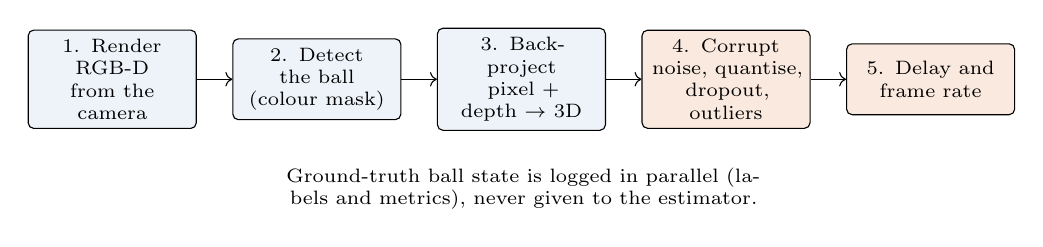
\begin{tikzpicture}[font=\scriptsize, node distance=0.45cm,
 b/.style={draw, rounded corners=2pt, align=center, minimum height=0.9cm, text width=1.9cm, fill=cblue!8}]
\node[b] (a) {1. Render RGB-D\\from the camera};
\node[b, right=of a] (b2) {2. Detect the ball\\(colour mask)};
\node[b, right=of b2] (c) {3. Back-project\\pixel + depth $\to$ 3D};
\node[b, right=of c, fill=corange!15] (d) {4. Corrupt\\noise, quantise,\\dropout, outliers};
\node[b, right=of d, fill=corange!15] (e) {5. Delay and\\frame rate};
\draw[->] (a)--(b2); \draw[->] (b2)--(c); \draw[->] (c)--(d); \draw[->] (d)--(e);
\node[below=0.35cm of c, text width=9cm, align=center] {Ground-truth ball state is logged in parallel (labels and metrics), never given to the estimator.};
\end{tikzpicture}
\caption{The simulated sensor as a chain of stages. Orange stages are where the survey says
simulators are too clean.}
\end{figure}

\subsection{Geometry of the first scene \textnormal{(proposal)}}
Camera mounted above the floor looking straight down, height $H=3$ m, vertical field of view
$60^{\circ}$, image $640\times480$. Then:
\begin{itemize}
\item Focal length in pixels $f=\tfrac{480/2}{\tan 30^{\circ}}\approx 416$ px.
\item Floor footprint of one pixel $\approx \tfrac{2\cdot3\cdot\tan30^{\circ}}{480}\approx 7.2$ mm.
\item The ball diameter is $60$ mm, so it covers about $8$ pixels: this is the \emph{tiny-object
regime} of the racquetball papers (8--62 px), not an easy large target.
\item At $5$ m/s and $60$ Hz the ball moves $8.3$ cm $\approx 11.5$ px between frames.
\end{itemize}

\subsection{Back-projection (pixel to 3D point)}
For a pixel $(u,v)$ with depth $Z$ and principal point $(c_x,c_y)$:
\[
X=\frac{(u-c_x)\,Z}{f},\qquad Y=\frac{(v-c_y)\,Z}{f},\qquad Z=Z .
\]
Then the camera-frame point is transformed to the world frame with the camera pose.

\subsection{Three small details that cause large errors}
\begin{enumerate}
\item \textbf{Depth buffer is not metres.} A rendered depth buffer stores a non-linear value in
$[0,1]$ that must be converted using the near and far clipping planes
(for a standard perspective buffer $Z=\dfrac{z_{\mathrm{near}}z_{\mathrm{far}}}
{z_{\mathrm{far}}-d\,(z_{\mathrm{far}}-z_{\mathrm{near}})}$). \emph{I will check the exact MuJoCo
convention in code before relying on this formula.}
\item \textbf{Surface versus centre.} The depth at the ball's centre pixel measures the
\emph{top surface}, which is one radius ($3$ cm) closer to the camera than the ball's centre. If we
do not add $r$ we create a constant $3$ cm bias in height (and a smaller bias in $x,y$ off the axis).
\item \textbf{The ground truth must match the same point.} The estimator is compared to the ball
\emph{centre}, so the detector pipeline must output a centre estimate, not a surface point.
\end{enumerate}

\subsection{Corruption stage: parameter table}
\begin{center}
\renewcommand{\arraystretch}{1.25}
\begin{tabularx}{\textwidth}{@{}l X X@{}}
\toprule
Effect & Model & Source / status \\
\midrule
range-dependent noise & $\sigma_Z=k\,Z^{2}$, Gaussian & shape: paper 12; $k$ \emph{placeholder} (e.g.\ $10^{-3}$\,m$^{-1}$ gives $1$ mm at $1$ m, $9$ mm at $3$ m) \\
quantisation & round depth to a step (e.g.\ $1$ mm) & paper 10 (3.2.1); step \emph{placeholder} \\
lateral noise & centroid jitter of a fraction of a pixel & \emph{placeholder} \\
dropout / tracking loss & Bernoulli per frame, higher near edges and when occluded & paper 11 says it matters most; rate \emph{placeholder} \\
outliers & small probability of a wrong depth & paper 10 (non-Gaussian noise); \emph{placeholder} \\
latency & fixed (or random) $\tau$ & paper 11: about $40$ ms \\
frame rate & e.g.\ $30$ or $60$ Hz while physics runs at $200$ Hz & \emph{placeholder} \\
\bottomrule
\end{tabularx}
\end{center}

\subsection{Latency semantics}
Each measurement carries two times: the \textbf{capture time} $t_c$ (when the ball was where the
camera saw it) and the \textbf{arrival time} $t_c+\tau$ (when the estimator receives it). An
estimator that ignores this and treats the measurement as current is wrong by $v\,\tau$. With a
simple delay line this is easy to implement, and it gives the estimators a fair, identical
challenge.

\subsection{Validation tests before any experiment}
\begin{enumerate}
\item With all corruption off, the output equals the true position within half a pixel.
\item With only noise on, the empirical standard deviation matches $kZ^2$ at several heights.
\item The measured dropout fraction matches the chosen probability.
\item The delay between ground-truth time and delivery equals $\tau$ exactly.
\item The same random seed reproduces the same sensor stream.
\end{enumerate}

\subsection{Decisions needed from you before coding}
Camera height and resolution (proposal $3$ m, $640\times480$); frame rate; colour mask versus
depth-based sphere fit for the detector; the noise constant $k$; dropout model; delay value
(proposal $40$ ms).


% ============================================================ 11
\section{Test yourself}
\begin{enumerate}[label=\textbf{Q\arabic*.}]
\item \emph{What is the difference between the reality gap and the performance gap?}\\
The reality gap compares the two worlds (their dynamics and sensors). The performance gap compares
the score of one fixed policy in the two worlds. Only the second must be small for transfer.
\item \emph{Why is ``belief'' central to us?}\\
Because the robot never sees the true ball state; the estimator's output is the belief that the
planner will act on.
\item \emph{Name three things real depth sensors do that a basic Gaussian-noise simulator omits.}\\
Range-dependent noise, quantisation, missing data at edges and on small objects (also depth shadows
and ambient-light interference).
\item \emph{Why does the survey say slower motion reduces the gap, and why does that matter for us?}\\
Slow motion is less sensitive to modelling error, delay and noise. Our balls are fast, so delay and
noise will matter more.
\item \emph{Why can SRCC not be used in our project?}\\
It needs real-world scores to correlate with simulation scores; we have only simulation.
\item \emph{What is ``privileged information'' and how do we use it?}\\
Information available only in simulation (true ball state). We use it as the label for training
and as the reference for metrics, but never as an input to the planner in the estimation setting.
\item \emph{In the Bayes filter, which step lowers uncertainty and which raises it?}\\
The update step (it uses the measurement) lowers it; the predict step (it uses imperfect dynamics) raises it.
\item \emph{Why does a position-only camera give a velocity estimate?}\\
Because the filter's dynamics link position and velocity; a position that moved more than predicted corrects the velocity (toy example in Deep dive A).
\item \emph{Why can $D_{\mathrm{KL}}(\text{sim}\|\text{real})$ be small while the simulator is still dangerous?}\\
Because KL is asymmetric: if the simulator never produces an event that happens in reality (dropout), the reverse direction is infinite.
\item \emph{Why must a $92.5\%$ versus $89.8\%$ difference over $200$ launches be treated with care?}\\
The standard error is about $2$ points, so the difference is within noise unless a paired test is used.
\item \emph{Why add the ball radius to the measured depth?}\\
Depth at the centre pixel measures the top surface, one radius closer than the ball's centre.
\end{enumerate}

\appendix
\section{Symbol cheat sheet}
\begin{center}
\renewcommand{\arraystretch}{1.2}
\begin{tabularx}{\textwidth}{@{}l X@{}}
\toprule
Symbol & Meaning \\
\midrule
$M=(\mathcal S,\mathcal A,T,R,\mathcal Z,O,\gamma)$ & POMDP tuple \\
$s_t,\ a_t,\ z_t$ & state, action, observation at time $t$ \\
$b_t$ & belief (distribution over states) \\
$\pi$ & policy: belief $\to$ action \\
$T_r,\ O_r$ / $T_s,\ O_s$ & real / simulated dynamics and observation model \\
$D$ & divergence between distributions \\
$G_{\mathrm{dyn}},\ G_{\mathrm{perc}}$ & dynamics gap, perception gap \\
$J_M(\pi)$ & expected return of $\pi$ in world $M$ \\
$G_{\mathrm{perf}}$ & performance gap $=|J_{M_s}(\pi)-J_{M_r}(\pi)|$ \\
SRCC & sim-to-real correlation coefficient (Pearson) \\
$E_{\mathrm{replay}}$ & offline replay error \\
\bottomrule
\end{tabularx}
\end{center}

\section{Where each part is in the paper}
\begin{center}
\renewcommand{\arraystretch}{1.2}
\begin{tabularx}{\textwidth}{@{}l X@{}}
\toprule
Paper section & Content (this guide) \\
\midrule
1 Introduction & benefits, the problem, roadmap (Section 3 of this guide) \\
2 Preliminaries & POMDP, simulation, reality and performance gap (Section 4) \\
3 Sources of the gap & dynamics, perception, actuation, system design (Section 5) \\
4 Existing solutions & recipe, reducing, overcoming (Section 6) \\
5 Evaluation metrics & SRCC, replay error, visual fidelity, success rate (Section 7) \\
6 Discussion & open problems (Section 8) \\
7 Conclusion & not covered (one paragraph) \\
\bottomrule
\end{tabularx}
\end{center}

\end{document}
